\documentclass[11pt,a4paper]{article}
\usepackage[utf8]{inputenc}
\usepackage[margin=1in]{geometry}
\usepackage{amsmath}
\usepackage{amssymb}
\usepackage{hyperref}
\usepackage{graphicx}
\usepackage{listings}
\usepackage{xcolor}
\usepackage{tikz}
\usepackage{algorithm}
\usepackage{algpseudocode}

\definecolor{codegreen}{rgb}{0,0.6,0}
\definecolor{codegray}{rgb}{0.5,0.5,0.5}
\definecolor{codepurple}{rgb}{0.58,0,0.82}
\definecolor{backcolour}{rgb}{0.95,0.95,0.92}

\lstdefinestyle{rust}{
    backgroundcolor=\color{backcolour},
    commentstyle=\color{codegreen},
    keywordstyle=\color{magenta},
    numberstyle=\tiny\color{codegray},
    stringstyle=\color{codepurple},
    basicstyle=\ttfamily\footnotesize,
    breakatwhitespace=false,
    breaklines=true,
    captionpos=b,
    keepspaces=true,
    numbers=left,
    numbersep=5pt,
    showspaces=false,
    showstringspaces=false,
    showtabs=false,
    tabsize=2
}

\lstset{style=rust}

\title{\textbf{Q-NarwhalKnight Testnet Bounty Protocol} \\
\large Trust-Minimized Reward System with Post-Quantum Security}
\author{Q-NarwhalKnight Core Engineering Team}
\date{Version 1.0 -- \today}

\begin{document}

\maketitle

\begin{abstract}
We present the \textit{Q-NarwhalKnight Testnet Bounty Protocol}, a cryptographically secure and Sybil-resistant reward system designed to incentivize comprehensive testnet participation. The protocol combines (a) a Rust services backend with RocksDB storage for testnet activity tracking; (b) AEGIS-QL post-quantum access control for administrative operations; (c) a weighted scoring engine with fraud detection across five activity categories; (d) Merkle tree-based mainnet reward distribution; and (e) a Vite/React dApp for user participation tracking. The system rewards genuine contributions while preventing gaming through multi-layered fraud detection, achieving fair distribution of mainnet tokens to early adopters who meaningfully contribute to network robustness.
\end{abstract}

\tableofcontents
\newpage

\section{Introduction}

\subsection{Motivation}
Successful blockchain mainnet launches require:
\begin{itemize}
    \item \textbf{Robust Testing}: Comprehensive stress testing, bug discovery, and performance validation
    \item \textbf{Community Engagement}: Loyal early adopters with technical expertise
    \item \textbf{Network Resilience}: Real-world testing of consensus, networking, and economic models
    \item \textbf{Fair Distribution}: Transparent reward mechanisms that prevent gaming
\end{itemize}

Traditional testnet participation often lacks clear incentive structures, leading to low engagement and insufficient testing coverage. We address this through a trust-minimized bounty protocol with cryptographic guarantees.

\subsection{System Overview}

The protocol operates in two phases:

\textbf{Phase 1 (Testnet)}: Continuous activity tracking, scoring, and leaderboard updates \\
\textbf{Phase 2 (Mainnet)}: Merkle-proof-based token distribution with vesting schedules

\begin{figure}[h]
\centering
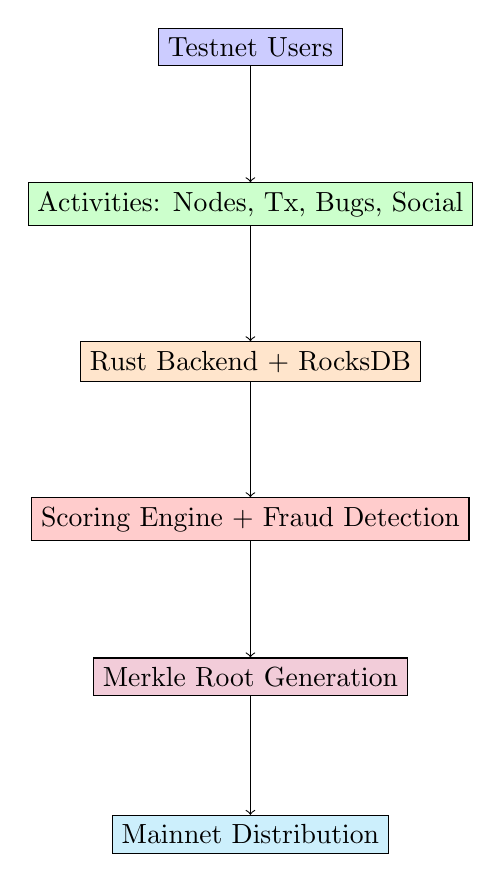
\begin{tikzpicture}[node distance=2cm]
\node (user) [rectangle, draw, fill=blue!20] {Testnet Users};
\node (activities) [rectangle, draw, fill=green!20, below of=user] {Activities: Nodes, Tx, Bugs, Social};
\node (backend) [rectangle, draw, fill=orange!20, below of=activities] {Rust Backend + RocksDB};
\node (scoring) [rectangle, draw, fill=red!20, below of=backend] {Scoring Engine + Fraud Detection};
\node (merkle) [rectangle, draw, fill=purple!20, below of=scoring] {Merkle Root Generation};
\node (mainnet) [rectangle, draw, fill=cyan!20, below of=merkle] {Mainnet Distribution};

\draw[->] (user) -- (activities);
\draw[->] (activities) -- (backend);
\draw[->] (backend) -- (scoring);
\draw[->] (scoring) -- (merkle);
\draw[->] (merkle) -- (mainnet);
\end{tikzpicture}
\caption{Testnet Bounty Protocol Architecture}
\end{figure}

\section{Core Concepts}

\subsection{Identity Binding}

Users register their testnet wallet and optionally bind to a mainnet wallet for future reward claims:

\begin{lstlisting}[language=rust]
pub struct TestnetUser {
    pub user_id: Uuid,
    pub testnet_address: [u8; 32],       // QNK testnet address
    pub mainnet_address: Option<[u8; 32]>, // Mainnet binding
    pub social_accounts: SocialAccounts,  // GitHub, X, Discord
    pub tier: BountyTier,                 // Reward tier
    pub total_score: f64,                 // Accumulated score
}
\end{lstlisting}

\subsection{Bounty Tiers}

Four tiers based on contribution percentile:

\begin{table}[h]
\centering
\begin{tabular}{|l|l|l|l|}
\hline
\textbf{Tier} & \textbf{Percentile} & \textbf{Reward Pool \%} & \textbf{Vesting} \\ \hline
Pioneer       & Top 1\%              & 20\%                     & 6 months         \\ \hline
Contributor   & Top 10\%             & 30\%                     & 3 months         \\ \hline
Participant   & Top 50\%             & 40\%                     & 1 month          \\ \hline
Supporter     & All valid            & 10\%                     & None             \\ \hline
\end{tabular}
\caption{Bounty Tier Structure}
\end{table}

\section{Scoring System}

\subsection{Weighted Formula}

The final score combines five weighted categories with multipliers:

\begin{equation}
\text{FinalScore}_u = \text{BaseScore}_u \times \text{EarlyMult} \times \text{ConsistencyBonus}
\end{equation}

Where:

\begin{equation}
\begin{split}
\text{BaseScore}_u = & \ 0.30 \times f_{\text{node}}(\text{NodeOps}_u) \\
                    & + 0.25 \times f_{\text{tx}}(\text{TxVolume}_u) \\
                    & + 0.20 \times f_{\text{bug}}(\text{BugReports}_u) \\
                    & + 0.15 \times \text{Community}_u \\
                    & + 0.10 \times \text{Social}_u
\end{split}
\end{equation}

\subsection{Activity Categories}

\begin{table}[h]
\centering
\begin{tabular}{|l|l|l|l|}
\hline
\textbf{Category} & \textbf{Weight} & \textbf{Max Points} & \textbf{Key Factors} \\ \hline
Node Operations   & 30\%            & 300                 & Uptime, blocks, governance \\ \hline
Transactions      & 25\%            & 250                 & Volume, diversity, DeFi usage \\ \hline
Bug Reports       & 20\%            & 200                 & Severity, quality, fixes \\ \hline
Community         & 15\%            & 150                 & Docs, tutorials, support \\ \hline
Social Media      & 10\%            & 100                 & Education, awareness \\ \hline
\end{tabular}
\caption{Activity Category Weights}
\end{table}

\subsubsection{Node Operations Scoring}

\begin{equation}
f_{\text{node}}(\text{metrics}) = 0.4 \times S_{\text{uptime}} + 0.3 \times S_{\text{blocks}} + 0.2 \times S_{\text{votes}} + 0.1 \times S_{\text{peers}}
\end{equation}

Where each component is normalized to its maximum value:
\begin{itemize}
    \item $S_{\text{uptime}} = \frac{\text{avg\_uptime}}{100} \times 120$
    \item $S_{\text{blocks}} = \min\left(\frac{\text{total\_blocks}}{1000}, 1\right) \times 90$
    \item $S_{\text{votes}} = \min\left(\frac{\text{governance\_votes}}{100}, 1\right) \times 60$
    \item $S_{\text{peers}} = \min\left(\frac{\text{avg\_peers}}{50}, 1\right) \times 30$
\end{itemize}

\subsubsection{Transaction Scoring}

\begin{equation}
f_{\text{tx}}(\text{txs}) = 0.4 \times S_{\text{count}} + 0.3 \times S_{\text{value}} + 0.2 \times S_{\text{contracts}} + 0.1 \times S_{\text{swaps}}
\end{equation}

\subsubsection{Bug Report Scoring}

Bug reports are severity-weighted:

\begin{table}[h]
\centering
\begin{tabular}{|l|l|l|}
\hline
\textbf{Severity} & \textbf{Multiplier} & \textbf{Pool Allocation} \\ \hline
Critical          & 100.0x              & 10\% of bounty pool      \\ \hline
High              & 50.0x               & 5\% of bounty pool       \\ \hline
Medium            & 20.0x               & 2\% of bounty pool       \\ \hline
Low               & 10.0x               & 1\% of bounty pool       \\ \hline
\end{tabular}
\caption{Bug Severity Scoring}
\end{table}

\subsection{Multipliers}

\subsubsection{Early Participation Multiplier}

Rewards early testers with exponentially declining bonuses:

\begin{equation}
\text{EarlyMult}(t) = 1.0 + 0.5 \times \left(\frac{t}{30}\right)^{-0.5}
\end{equation}

Where $t$ is days since campaign start. This yields:
\begin{itemize}
    \item Day 1: 2.0x multiplier
    \item Day 7: 1.6x multiplier
    \item Day 14: 1.4x multiplier
    \item Day 30+: 1.0x multiplier
\end{itemize}

\subsubsection{Consistency Bonus}

Rewards sustained participation over sporadic activity:

\begin{equation}
\text{ConsistencyBonus} = 1.0 + 0.2 \times \frac{\text{active\_days}}{\text{total\_days}}
\end{equation}

Ranges from 1.0x (no consistency) to 1.2x (daily participation).

\section{Fraud Detection}

\subsection{Wash Trading Detection}

Identifies suspicious transaction patterns through variance analysis:

\begin{algorithm}
\caption{Wash Trading Detection}
\begin{algorithmic}[1]
\State $\text{txs} \gets \text{user\_transactions}$
\If{$|\text{txs}| < 10$}
    \State \Return $\textbf{false}$ \Comment{Insufficient data}
\EndIf
\State $\text{values} \gets [\text{tx.value} \mid \text{tx} \in \text{txs}]$
\State $\mu \gets \text{mean}(\text{values})$
\State $\sigma^2 \gets \text{variance}(\text{values})$
\If{$\sigma^2 < 0.1 \times \mu$}
    \State \Return $\textbf{true}$ \Comment{Low variance suggests wash trading}
\Else
    \State \Return $\textbf{false}$
\EndIf
\end{algorithmic}
\end{algorithm}

Detected wash traders incur a \textbf{70\% score penalty}.

\subsection{Social Media Spam Detection}

Identifies bot-like activity through time clustering and engagement analysis:

\begin{itemize}
    \item \textbf{Time Clustering}: $>$50 posts in 24 hours flagged
    \item \textbf{Low Engagement}: Average engagement $<$0.1 suggests bots
    \item \textbf{Content Duplication}: Repetitive patterns detected via hashing
\end{itemize}

Detected spam incurs an \textbf{80\% score penalty}.

\subsection{Node Sybil Resistance}

\begin{itemize}
    \item \textbf{IP Analysis}: Geographic clustering detection
    \item \textbf{Hardware Fingerprinting}: Identical machine signatures flagged
    \item \textbf{Unrealistic Metrics}: $>$99.9\% uptime + $>$10k blocks flagged
\end{itemize}

Suspicious nodes receive a \textbf{50\% score penalty}.

\section{AEGIS-QL Access Control}

Administrative operations (leaderboard building, campaign finalization, Merkle root publication) require AEGIS-QL post-quantum signatures.

\subsection{Cryptographic Foundation}

AEGIS-QL (Asymmetric Efficient Graph-based Integer System with Quantum Resistance) is based on \textbf{sparse Ring-LWE} with optimized Number Theoretic Transform (NTT) operations:

\begin{itemize}
    \item \textbf{Security Level}: 256-bit classical, 128-bit quantum
    \item \textbf{Polynomial Degree}: 512 (optimized for 50-67\% faster operations than Kyber-768)
    \item \textbf{Modulus}: 12289 (NTT-friendly prime: $12289 = 24 \times 512 + 1$)
    \item \textbf{Sparse Graph Degree}: 8 (reduces $O(n^2)$ to $O(k \cdot n)$)
    \item \textbf{Signature Size}: ~1.5KB
    \item \textbf{Public Key Size}: ~800 bytes
\end{itemize}

The system provides horizontal scalability with linear throughput scaling across workers, making it ideal for high-frequency administrative operations in distributed bounty systems.

\subsection{Access Levels}

\begin{table}[h]
\centering
\begin{tabular}{|l|p{8cm}|}
\hline
\textbf{Level} & \textbf{Permissions} \\ \hline
Founder        & Full control: campaign creation, reward pool allocation, Merkle root publication \\ \hline
Admin          & Leaderboard building, user verification, tier adjustments \\ \hline
Operator       & Activity verification, bug report validation \\ \hline
User           & Self-service: registration, score viewing, mainnet binding \\ \hline
\end{tabular}
\caption{AEGIS-QL Access Control Hierarchy}
\end{table}

\subsection{Signature Verification}

\begin{lstlisting}[language=rust]
pub fn verify_access(
    &self,
    wallet_address: &[u8; 32],
    signature: &Signature,
    message: &[u8],
    required_level: AccessLevel,
) -> Result<bool, AegisError> {
    // Find wallet in ACL
    let entry = self.acl.iter()
        .find(|e| &e.wallet_address == wallet_address)
        .ok_or(AegisError::Unauthorized)?;

    // Check access level hierarchy
    if !Self::has_access(entry.access_level, required_level) {
        return Err(AegisError::Unauthorized);
    }

    // Verify AEGIS-QL post-quantum signature
    self.aegis.verify(message, signature, &entry.public_key)
}
\end{lstlisting}

\section{Storage Architecture}

\subsection{RocksDB Column Families}

\begin{table}[h]
\centering
\begin{tabular}{|l|p{8cm}|}
\hline
\textbf{Column Family} & \textbf{Contents} \\ \hline
\texttt{testnet\_users} & User registrations, wallet bindings, social accounts \\ \hline
\texttt{node\_metrics} & Uptime, blocks produced, governance votes, timestamps \\ \hline
\texttt{transactions} & Transaction hashes, values, contract interactions, DEX swaps \\ \hline
\texttt{bug\_reports} & GitHub URLs, severity levels, verification status, bounties \\ \hline
\texttt{community\_contributions} & Documentation, tutorials, impact scores \\ \hline
\texttt{social\_activities} & Platform, activity type, engagement scores, verification \\ \hline
\texttt{final\_scores} & Total scores, category breakdowns, ranks, Merkle proofs \\ \hline
\texttt{campaigns} & Campaign metadata, reward pools, Merkle roots \\ \hline
\texttt{leaderboard} & Cached rankings for fast queries \\ \hline
\end{tabular}
\caption{RocksDB Storage Schema}
\end{table}

\subsection{Caching Strategy}

\begin{itemize}
    \item \textbf{User Cache}: DashMap for O(1) user lookups
    \item \textbf{Leaderboard Cache}: RwLock-protected Vec for fast leaderboard queries
    \item \textbf{Write-Through}: All modifications persist to RocksDB immediately
    \item \textbf{Cache Invalidation}: On score updates, tier recalculations, campaign finalization
\end{itemize}

\section{Merkle Tree Distribution}

\subsection{Construction}

After testnet conclusion, a Merkle tree is built from final scores:

\begin{algorithm}
\caption{Merkle Tree Construction}
\begin{algorithmic}[1]
\State $\text{users} \gets \text{get\_all\_users\_sorted\_by\_score()}$
\State $\text{leaves} \gets []$
\ForAll{$\text{user} \in \text{users}$}
    \State $\text{leaf} \gets \text{hash}(\text{user.address} \parallel \text{user.reward\_amount})$
    \State $\text{leaves.append}(\text{leaf})$
\EndFor
\State $\text{tree} \gets \text{MerkleTree::new}(\text{leaves})$
\State $\text{root} \gets \text{tree.root()}$
\State \textbf{publish\_to\_mainnet}$(\text{root})$
\State \Return $\text{tree}$
\end{algorithmic}
\end{algorithm}

\subsection{Claim Process}

On mainnet launch, users claim rewards with Merkle proofs:

\begin{lstlisting}[language=rust]
pub fn claim_bounty(
    bounty_id: BountyId,
    amount: u64,
    merkle_proof: Vec<[u8; 32]>,
) -> Result<(), BountyError> {
    let merkle_root = get_bounty_merkle_root(bounty_id)?;
    let leaf = hash(&(caller_address, amount));

    // Verify Merkle proof
    if !verify_merkle_proof(&leaf, &merkle_proof, &merkle_root) {
        return Err(BountyError::InvalidProof);
    }

    // Transfer tokens with vesting
    transfer_with_vesting(caller_address, amount, user_tier.vesting_months())
}
\end{lstlisting}

\section{API Endpoints}

\subsection{REST API}

\begin{table}[h]
\centering
\small
\begin{tabular}{|l|l|p{5cm}|}
\hline
\textbf{Method} & \textbf{Endpoint} & \textbf{Description} \\ \hline
POST & \texttt{/v1/testnet/register} & Register testnet wallet \\ \hline
POST & \texttt{/v1/testnet/bind-mainnet} & Bind mainnet wallet \\ \hline
GET & \texttt{/v1/testnet/score} & Get current score breakdown \\ \hline
GET & \texttt{/v1/testnet/leaderboard} & Current rankings (paginated) \\ \hline
POST & \texttt{/v1/bug-report} & Submit bug report with proof \\ \hline
POST & \texttt{/v1/social/verify} & Verify social media accounts \\ \hline
GET & \texttt{/v1/bounty/claim-status} & Mainnet claim readiness \\ \hline
POST & \texttt{/v1/admin/build-leaderboard} & Rebuild leaderboard cache (Admin) \\ \hline
POST & \texttt{/v1/founder/finalize-campaign} & Generate Merkle root (Founder) \\ \hline
\end{tabular}
\caption{Bounty Protocol REST API}
\end{table}

\subsection{WebSocket Streams}

Real-time updates for:
\begin{itemize}
    \item \texttt{/ws/leaderboard} -- Live ranking changes
    \item \texttt{/ws/scores} -- Personal score updates
    \item \texttt{/ws/campaign-events} -- Campaign milestones
\end{itemize}

\section{Frontend dApp}

\subsection{Technology Stack}

\begin{itemize}
    \item \textbf{Framework}: Vite + React + TypeScript
    \item \textbf{Styling}: Tailwind CSS with quantum-themed palette
    \item \textbf{Charts}: Chart.js for score visualizations
    \item \textbf{Wallet}: Multi-wallet support (MetaMask, WalletConnect)
    \item \textbf{Real-time}: Server-Sent Events (SSE) for live updates
\end{itemize}

\subsection{Key Screens}

\begin{enumerate}
    \item \textbf{Registration Wizard}: Step-by-step testnet/mainnet wallet binding
    \item \textbf{Score Dashboard}: Real-time scoring with category breakdown charts
    \item \textbf{Leaderboard}: Live rankings with tier badges and filtering
    \item \textbf{Activity Monitor}: Node status, transaction history, bug report tracking
    \item \textbf{Bounty Board}: Special bounties with progress tracking
    \item \textbf{Social Integration}: OAuth flows for Twitter, GitHub, Discord
    \item \textbf{Claim Assistant}: Mainnet reward claiming with gas optimization
\end{enumerate}

\section{Economic Sustainability}

\subsection{Token Allocation}

\begin{itemize}
    \item \textbf{Bounty Pool}: 2-5\% of total token supply
    \item \textbf{Early Adopter Rewards}: 50\% of bounty pool (Pioneer 20\% + Contributor 30\%)
    \item \textbf{General Participation}: 50\% of bounty pool (Participant 40\% + Supporter 10\%)
    \item \textbf{Vesting}: Aligns long-term incentives with project success
\end{itemize}

\subsection{Unclaimed Token Handling}

\begin{itemize}
    \item \textbf{Claim Window}: 90 days from mainnet launch
    \item \textbf{Unclaimed Tokens}: Return to DAO treasury
    \item \textbf{Gas Compensation}: Partial gas refund for claim transactions
\end{itemize}

\section{Security Considerations}

\subsection{Threat Model}

\begin{itemize}
    \item \textbf{Sybil Attacks}: Multi-account detection via IP clustering and hardware fingerprinting
    \item \textbf{Wash Trading}: Transaction pattern analysis with variance thresholds
    \item \textbf{Social Spam}: Time clustering and engagement quality metrics
    \item \textbf{Bug Inflation}: Duplicate detection and community verification
    \item \textbf{Claim Frontrunning}: Merkle proofs prevent proof manipulation
\end{itemize}

\subsection{Post-Quantum Security}

\begin{itemize}
    \item \textbf{AEGIS-QL Signatures}: 256-bit classical, 128-bit quantum security
    \item \textbf{Merkle Trees}: SHA3-256 resistant to quantum attacks
    \item \textbf{Identity Binding}: Post-quantum secure wallet associations
\end{itemize}

\section{Implementation Roadmap}

\subsection{Phase 1: Core Infrastructure (Weeks 1-2)}
\begin{itemize}
    \item Rust crate development (\texttt{q-bounty-protocol})
    \item RocksDB storage layer with AEGIS-QL integration
    \item Scoring engine with fraud detection
\end{itemize}

\subsection{Phase 2: Activity Tracking (Weeks 2-3)}
\begin{itemize}
    \item Node metrics collector (Prometheus-based)
    \item Transaction scanner (blockchain RPC integration)
    \item Bug report integrator (GitHub API)
    \item Social activity monitor (Twitter/GitHub/Discord APIs)
\end{itemize}

\subsection{Phase 3: API \& Frontend (Weeks 4-6)}
\begin{itemize}
    \item REST API development with Axum framework
    \item WebSocket real-time streams
    \item Vite/React dApp with Tailwind CSS
    \item Social OAuth integration flows
\end{itemize}

\subsection{Phase 4: Testnet Launch (Week 6)}
\begin{itemize}
    \item Bounty campaign initialization
    \item Public participation begins
    \item Real-time leaderboard updates
    \item Weekly progress reports
\end{itemize}

\subsection{Phase 5: Mainnet Preparation (Weeks 10-12)}
\begin{itemize}
    \item Final score calculation
    \item Merkle tree generation
    \item Smart contract deployment (mainnet)
    \item Claim system testing
\end{itemize}

\subsection{Phase 6: Mainnet Distribution (Week 13+)}
\begin{itemize}
    \item Reward distribution system activation
    \item User claim window opens (90 days)
    \item Vesting schedules begin
    \item Post-distribution analytics
\end{itemize}

\section{Success Metrics}

\begin{itemize}
    \item \textbf{Participation Rate}: $>$70\% of testnet nodes enrolled
    \item \textbf{Bug Discovery}: $>$100 valid bug reports, $>$10 critical issues
    \item \textbf{Community Growth}: $>$50\% increase in developer community
    \item \textbf{Network Stress}: Successfully handle 1M+ test transactions
    \item \textbf{Mainnet Readiness}: Zero critical bugs in production code
\end{itemize}

\section{Conclusion}

The Q-NarwhalKnight Testnet Bounty Protocol provides a cryptographically secure, Sybil-resistant framework for incentivizing comprehensive testnet participation. By combining:

\begin{itemize}
    \item \textbf{Weighted Scoring}: Fair evaluation across five activity categories
    \item \textbf{Fraud Detection}: Multi-layered anti-gaming controls
    \item \textbf{Post-Quantum Security}: AEGIS-QL access control and Merkle proofs
    \item \textbf{Transparent Distribution}: Verifiable Merkle tree-based claims
\end{itemize}

We enable fair, transparent, and secure reward distribution to early adopters who meaningfully contribute to network robustness. The protocol's design ensures alignment between testnet participation incentives and long-term project success.

\section*{Acknowledgments}

This protocol was developed by the Q-NarwhalKnight Core Engineering Team with inspiration from testnet incentive programs across the blockchain ecosystem. Special thanks to the DAG-BFT consensus research community and post-quantum cryptography standards from NIST.

\end{document}
